\begin{prob}
    Topologically sort the vertices of the following graph. Note that there
    may be multiple, equally-correct topological sorts.

    You do not need to show your work for this problem.

    \vspace{1em}

    \begin{center}
        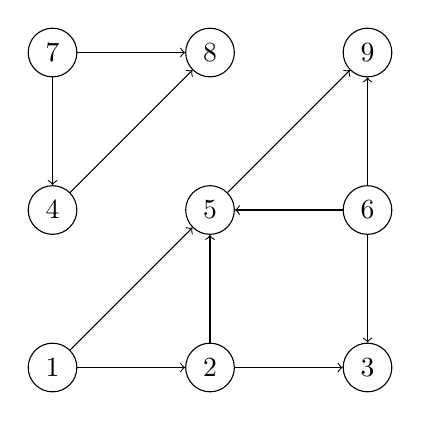
\begin{tikzpicture}
            \foreach \i in {1,...,9}{
                \pgfmathparse{mod(\i-1,3)} \pgfmathresult %displays 2.0
                \pgfmathtruncatemacro{\x}{\pgfmathresult}  

                \pgfmathtruncatemacro{\y}{(\i-1)/3}

                \node[draw, circle] (n\i) at (2*\x, 2*\y) {$\i$}; 
            }

            \foreach \u/\v in {%
                2/3,
                2/5,
                5/9,
                6/5,
                4/8,
                7/4,
                7/8,
                1/5,
                6/9,
                6/3,
                1/2%
                }{
                \draw (n\u) edge[->] (n\v);
            }
        \end{tikzpicture}
    \end{center}

    \begin{soln}
        Our algorithm for producing a topological sort of the nodes is to 
        first perform a DFS in order to record finish times, and then to
        sort the nodes in order of decreasing finish time.

        If we start a DFS at node 1 and us the convention that the neighbors
        are produced in increasing order of label, we will visit nodes 1, 2, 3,
        5, and 9. This search didn't visit all of the nodes of the graph, so
        suppose we restart the search at node 6. This search will not move away
        from 6, and so we restart the search again at node 7, visiting nodes 4 and 8.
        The finish times resulting from this search are
        \inputminted{python}{\thisdir/include-solution/topo_answer.py}

        Ordering these by decreasing finish time, we obtain a topological sort of:
        \[
            7, 4, 8, 6, 1, 2, 5, 9, 3.
        \]

        Your topological sort may be different, but still correct. This may happen
        if you restarted the search at different nodes than what was used above.
    \end{soln}

\end{prob}
